
\begin{His}
Les origines de la trigonométrie remontent aux civilisations d’Égypte antique, de Mésopotamie et de la vallée de l’Indus, il y a plus de 4 000 ans. Il semblerait que les Babyloniens aient basé la trigonométrie sur un système numérique à base 60. \textsc{Lagadha} (ca -1350 ; ca -1200) aurait été le premier mathématicien à utiliser la géométrie et la trigonométrie pour l’astronomie et dont on retrouve une trace écrite ; la plupart de ses travaux aurait aujourd’hui disparu, mais son Vedanga Jyotisha nous est parvenu.

La première utilisation du sinus apparaît dans les Sulba Sutras en Inde, entre ca -800 et ca -500, où le sinus de $\pi/4$ (ou $45\deg$) est correctement calculé comme $1/\sqrt{2}$ dans un problème de construction d’un cercle de même aire qu’un carré donné (le contraire de la quadrature du cercle).

\vspace{0.4cm}

\textbf{Les astronomes grecs}

L'astronome et mathématicien grec Hipparque de \textsc{Nicée} (-190 ; -120) construisit les premières tables trigonométriques sous la forme de tables de cordes : elles faisaient correspondre à chaque valeur de l'angle au centre (avec une division du cercle en $360\deg$), la longueur de la corde interceptée dans le cercle, pour un rayon fixe donné. Ce calcul correspond au double du sinus de l'angle moitié, et donne donc, d'une certaine façon, ce que nous appelons aujourd'hui une table de sinus. Toutefois, les tables d'\textsc{Hipparque} n'étant pas parvenues jusqu'à nous, elles ne nous sont connues que par le grec \textsc{Ptolémée}, qui les publia, vers l'an 150, avec leur mode de construction dans son Almageste. C'est ainsi qu'elles furent redécouvertes à la fin du Moyen Âge par Georg von \textsc{Purbach} et son élève \textsc{Regiomontanus}. On attribue à \textsc{Ménélaos d'Alexandrie} (fin du Ier siècle) des développements en trigonométrie sphérique, au moins partiellement présents dans l'Almageste et longtemps attribués à \textsc{Ptolémée} lui-même.

Le mathématicien indien \textsc{Âryabhata}, en 499, donne une table des sinus et des cosinus. Il utilise zya pour sinus, kotizya pour cosinus et otkram zya pour l'inverse du sinus. Il introduit aussi le sinus verse.

Un autre mathématicien indien, \textsc{Brahmagupta}, utilise en 628 l'interpolation numérique pour calculer la valeur des sinus jusqu'au second ordre.

\vspace{0.4cm}

\textbf{Essor dans le monde musulman}

C'est dans le monde musulman que la trigonométrie prend le statut de discipline à part entière et se détache de l'astronomie.
\vspace{0.2cm}
\begin{wrapfigure}[12]{r}{3.6cm}
\vspace{-7mm}
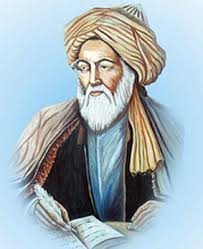
\includegraphics[scale=0.5]{image_chapitres/alkashi.jpg} 
\unnumberedcaption{Jamshid \textsc{Al-Kachi}}
\end{wrapfigure}
Omar \textsc{Khayyam} (1048-1131) combine l'utilisation de la trigonométrie et la théorie de l'approximation pour fournir des méthodes de résolutions d'équations algébriques par la géométrie. Des méthodes détaillées de constructions de tables de sinus et cosinus pour tous les angles sont écrites par le mathématicien \textsc{Bhāskara II} en 1150. Il développe aussi la trigonométrie sphérique. Au XIIIe siècle, Nasir al-Din \textsc{Tusi}, à la suite de \textsc{Bhāskara}, est probablement un des premiers à considérer la trigonométrie comme une discipline distincte des mathématiques. Enfin, au XIVe siècle, \textsc{\textbf{Al-Kachi}} réalise des tables de fonctions trigonométriques lors de ses études en astronomie.

\vspace{0.4cm}

\textbf{En Europe : redécouverte de Ptolémée}

En Europe, la trigonométrie se développe vers le milieu du XIVe siècle avec la traduction en latin des œuvres de Ptolémée. Les pionniers en ce domaine sont Georg von \textsc{Purbach} et surtout son étudiant \textsc{Regiomontanus}. Suivent au début du XVIe siècle les traités d'Oronce \textsc{Finé}, Pedro \textsc{Nunes} et Joachim \textsc{Rheticus}. Le mathématicien silésien Bartholomäus \textsc{Pitiscus} publie un travail remarquable sur la trigonométrie en 1595, dont le titre (Trigonometria) a donné son nom à la discipline. C'est le mathématicien flamand Adrien \textsc{Romain} qui introduit la notation moderne $sin \alpha$.

\vspace{0.4cm}
\textbf{Applications}

Les applications de la trigonométrie sont extrêmement nombreuses. En particulier, elle est utilisée en astronomie et en navigation avec notamment la technique de triangulation. Les autres champs où la trigonométrie intervient sont (liste non exhaustive) : physique, électricité, électronique, mécanique, acoustique, optique, statistiques, économie, biologie, chimie, médecine, météorologie, géodésie, géographie, cartographie, cryptographie, etc.

\PESP{https://fr.wikipedia.org/wiki/Trigonom\%C3\%A9trie}


\end{His}
